\chapter{Capstone Proposal: Team, Idea, and Feasibility}
\label{ch:proposal}

\noindent\fbox{\parbox{\dimexpr\linewidth-2\fboxsep-2\fboxrule}{%
\textbf{From zero:} No prerequisites. A \emph{capstone} is your final-year team project where you integrate everything from earlier courses to build a real system for a real stakeholder. We define every term---team role, proposal, feasibility---from scratch with intuition before formality. If you have never formed a project team or written a proposal, start here.}}
\vspace{0.4em}

\section*{Learning Outcomes}
After this chapter you will be able to:
\begin{enumerate}[label=(L\arabic*)]
    \item explain what a capstone project is and why it matters for your degree and career;
    \item form a balanced team, assign roles, and draft a team charter using Belbin insights;
    \item write a complete proposal covering problem, objectives, scope, and deliverables;
    \item evaluate feasibility via TELOS (Technical, Economic, Legal, Operational, Schedule);
    \item identify top risks and sketch a high-level timeline for a semester-long project.
\end{enumerate}

% ============================================================
\section{What Is a Capstone?}
\label{sec:what-capstone}

\textbf{Intuition.} Imagine you have taken programming, databases, networks, and software engineering as separate subjects. A capstone is the moment you stop solving textbook exercises and start solving a messy, open-ended problem for a real user---a clinic that needs appointment scheduling, a retailer that loses stock. Success is not just code that compiles; it is a system someone wants to use, delivered on time by a team that planned together.

\begin{definition}[Capstone Project]
A supervised, team-based project in the final year of study in which students conceive, plan, design, implement, test, and present a substantial computing artefact that addresses a stakeholder problem, demonstrating integration of prior learning and professional practice.
\end{definition}

Key traits: (i)~open-ended and stakeholder-driven, (ii)~team-based over one--two semesters, (iii)~assessed on process and product, not just code, (iv)~requires a written proposal, regular reviews, and a final demonstration and report. Assessment weights proposal quality because a flawed plan predicts a flawed product.

\begin{example}[Clinic Queue System]
Team of four proposes a QR-based queue for a polyclinic: patients scan on arrival, see live waiting time, and receive SMS when near turn. Problem: manual queues waste time and crowd waiting rooms. Objective: cut perceived wait by 30\% and halve no-shows. This one paragraph---problem plus measurable objective---is the kernel of every proposal in this chapter.
\end{example}

% ============================================================
\section{Team Formation}
\label{sec:team-formation}

Great proposals start with great teams. SC3099 teams are typically 3--5 members; diversity of skill and working style matters more than friendship.

\textbf{Core roles.} Every team needs coverage of four functions, often with one person covering two:
\begin{itemize}
    \item \textbf{Team Lead} --- owns planning, stakeholder communication, conflict resolution, and schedule.
    \item \textbf{Developer(s)} --- design and implement core features; manage repository and CI.
    \item \textbf{QA / Test Lead} --- defines test strategy, writes acceptance criteria, guards quality gates.
    \item \textbf{Designer} --- owns UX, wireframes, and presentation; ensures usability and accessibility.
\end{itemize}
Roles are not titles for hierarchy; they are \emph{accountabilities} that make decisions fast and avoid diffusion of responsibility.

\textbf{Belbin and balance.} Meredith Belbin identified nine team roles (e.g., Plant, Coordinator, Monitor-Evaluator, Implementer, Completer-Finisher). Healthy capstone teams balance \emph{thinking}, \emph{doing}, and \emph{social} roles. A team of four Plants generates ideas but ships nothing; a team of only Implementers ships fast but may solve the wrong problem. Use a short Belbin self-perception quiz at formation to spot gaps and negotiate who stretches into which role.

\textbf{Team charter.} Write a one-page charter on day one: shared goals, role assignments, meeting cadence, decision rule (e.g., majority after 24h async), tool stack, and conflict escalation (talk $\rightarrow$ mediator $\rightarrow$ supervisor). Sign it. Revisit it at each milestone.

\begin{figure}[h]
\centering
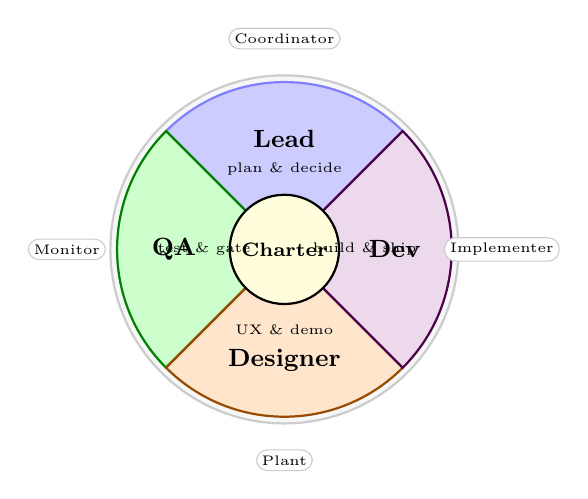
\begin{tikzpicture}[scale=0.85, every node/.style={font=\footnotesize}]
  % wheel background
  \draw[fill=gray!6,draw=gray!40,thick] (0,0) circle (2.6cm);
  % four role quadrants
  \fill[blue!20,draw=blue!50,thick] (0,0) -- (45:2.5cm) arc (45:135:2.5cm) -- cycle;
  \fill[green!20,draw=green!50!black,thick] (0,0) -- (135:2.5cm) arc (135:225:2.5cm) -- cycle;
  \fill[orange!20,draw=orange!60!black,thick] (0,0) -- (225:2.5cm) arc (225:315:2.5cm) -- cycle;
  \fill[violet!15,draw=violet!60!black,thick] (0,0) -- (315:2.5cm) arc (315:405:2.5cm) -- cycle;
  % centre hub
  \node[draw,circle,fill=yellow!14,minimum size=1.35cm,thick,align=center,font=\scriptsize\bfseries] at (0,0) {Charter};
  % role labels
  \node[align=center,font=\small\bfseries] at (90:1.65cm) {Lead};
  \node[align=center,font=\tiny] at (90:1.20cm) {plan \& decide};
  \node[align=center,font=\small\bfseries] at (180:1.65cm) {QA};
  \node[align=center,font=\tiny] at (180:1.20cm) {test \& gate};
  \node[align=center,font=\small\bfseries] at (270:1.65cm) {Designer};
  \node[align=center,font=\tiny] at (270:1.20cm) {UX \& demo};
  \node[align=center,font=\small\bfseries] at (0:1.65cm) {Dev};
  \node[align=center,font=\tiny] at (0:1.20cm) {build \& ship};
  % outer Belbin hints
  \node[font=\tiny,fill=white,draw=gray!40,rounded corners,inner sep=2pt] at (90:3.15cm) {Coordinator};
  \node[font=\tiny,fill=white,draw=gray!40,rounded corners,inner sep=2pt] at (180:3.25cm) {Monitor};
  \node[font=\tiny,fill=white,draw=gray!40,rounded corners,inner sep=2pt] at (270:3.15cm) {Plant};
  \node[font=\tiny,fill=white,draw=gray!40,rounded corners,inner sep=2pt] at (0:3.25cm) {Implementer};
\end{tikzpicture}
\caption{Team roles wheel: four accountabilities around a shared charter. Outer labels sample Belbin roles that complement each quadrant. Colour fills distinguish accountabilities; the centre reminds the team that charter commitments bind all segments.}
\label{fig:team-wheel}
\end{figure}

% ============================================================
\section{Proposal Structure}
\label{sec:proposal-structure}

A proposal is a promise phrased as a plan. Supervisors and stakeholders read it to decide whether your idea is worth funding with time and guidance. Every SC3099 proposal contains five sections:

\begin{description}
    \item[1. Problem Statement] Who hurts, how badly, and why existing solutions fail. One paragraph, evidence-backed.
    \item[2. Objectives] SMART goals (Specific, Measurable, Achievable, Relevant, Time-bound). ``Build an app'' is not SMART; ``reduce queue abandonment from 18\% to $<10$\% within 12 weeks'' is.
    \item[3. Scope] What is \emph{in} and explicitly \emph{out}. Scope creep kills capstones; write exclusion bullets.
    \item[4. Deliverables] Tangible artefacts: working system, test suite, user manual, demo video, final report.
    \item[5. Success Criteria] How you and the stakeholder will judge the outcome (metrics, acceptance tests).
\end{description}

Listing~1 shows a compact template you can copy into your repository and fill iteratively.

\begin{lstlisting}[language=Python,caption={Proposal skeleton as a Python dict---fill each value before your first supervisor meeting.},label={lst:proposal-template}]
proposal = {
    "title": "QR Queue for Polyclinic A",
    "problem": "Manual queues cause crowding; patients cannot estimate wait.",
    "stakeholder": "Nurse manager, Clinic A (interview 22 Aug)",
    "objectives": [
        "Cut perceived wait by 30% (survey, n>=50)",
        "Halve no-show rate to <8% via SMS nudge",
        "Deploy pilot in 1 clinic within 14 weeks"
    ],
    "scope": {
        "in_scope": ["QR check-in", "live ETA", "SMS nudge", "admin dashboard"],
        "out_scope": ["payment", "EHR integration", "iOS native app"]
    },
    "deliverables": ["web app", "test report", "user guide", "demo video"],
    "success_criteria": "80% of pilot users rate ETA as accurate; zero P1 defects at handover",
    "constraints": ["PDPA compliance", "max budget SGD 500", "NTU GitLab hosting"]
}
\end{lstlisting}

Write scope exclusions before you write features. Reviewers trust a team that says ``not in this semester'' more than one that promises everything.

% ============================================================
\section{Feasibility Analysis: TELOS}
\label{sec:feasibility}

Enthusiasm is necessary but not sufficient. TELOS forces honest feasibility across five lenses:
\begin{itemize}
    \item \textbf{T--Technical:} Do we have the stack, data, and skills? Can we prototype the riskiest slice in two weeks?
    \item \textbf{E--Economic:} Cost versus benefit. Cloud, devices, licences, and opportunity cost of team time.
    \item \textbf{L--Legal:} PDPA, copyright, licences, ethics approval, and stakeholder data agreements.
    \item \textbf{O--Operational:} Will users actually adopt it? Workflow fit, training, and support after handover.
    \item \textbf{S--Schedule:} Can a team of four deliver a usable increment in 13 weeks given exams and dependencies?
\end{itemize}
Score each lens 1--5. A proposal with any score $\le 2$ needs rework; two or more $\le 2$ is a no-go. Document assumptions explicitly---``hospital Wi-Fi is assumed available'' is cheaper to fix on paper than in week~10.

\begin{figure}[h]
\centering
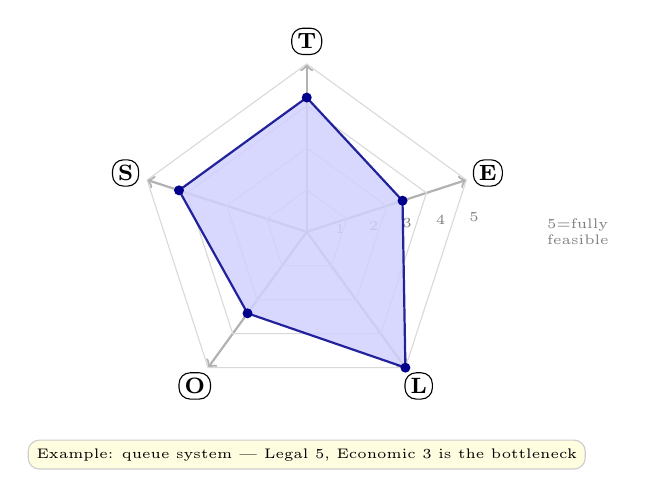
\begin{tikzpicture}[scale=0.82, every node/.style={font=\scriptsize}]
  % axes
  \coordinate (C) at (0,0);
  \foreach \a/\lbl in {90/T,18/E,306/L,234/O,162/S} {
    \draw[gray!60,thick,->] (C) -- (\a:2.6cm);
    \node[fill=white,draw,rounded corners,inner sep=2pt,font=\footnotesize\bfseries] at (\a:2.95cm) {\lbl};
  }
  % concentric grid
  \foreach \r in {0.65,1.3,1.95,2.6} {
    \draw[gray!30,thin] (90:\r) -- (18:\r) -- (306:\r) -- (234:\r) -- (162:\r) -- cycle;
  }
  \foreach \v in {1,2,3,4,5} \node[font=\tiny,gray] at (5:\v*0.52cm) {\v};
  % example scores: T4 E3 L5 O3 S4 (polyclinic queue)
  \fill[blue!18,draw=blue!55!black,thick,opacity=0.85]
    (90:2.08cm) -- (18:1.56cm) -- (306:2.6cm) -- (234:1.56cm) -- (162:2.08cm) -- cycle;
  \foreach \a/\r in {90/2.08,18/1.56,306/2.6,234/1.56,162/2.08} {
    \fill[blue!55!black] (\a:\r) circle (2.2pt);
  }
  \node[align=center,font=\tiny,fill=yellow!12,draw=gray!40,rounded corners,inner sep=3pt] at (0,-3.45cm) {Example: queue system --- Legal 5, Economic 3 is the bottleneck};
  \node[align=left,font=\tiny,gray] at (4.2,0) {5=fully\\feasible};
\end{tikzpicture}
\caption{TELOS radar: five feasibility axes scored 1--5. Shaded polygon shows the polyclinic example (Legal is strongest; Economic needs mitigation via free-tier hosting). Any axis $\le 2$ should block approval.}
\label{fig:telos-radar}
\end{figure}

If Economic scores 2 because SMS costs exceed budget, mitigate early: negotiate a free quota, switch to Telegram push, or reduce pilot size. Record the mitigation in the proposal; feasibility is a living judgement, not a one-time checkbox.

% ============================================================
\section{Risk and Timeline Preview}
\label{sec:risk-timeline}

Every proposal closes with risks and a high-level timeline. List the top five risks with likelihood, impact, and mitigation. Example risks: stakeholder unavailability, API deprecation, exam crunch in weeks~10--12, PDPA review delay, device procurement lag. For each, name an owner and a trigger date.

Timeline at proposal stage is coarse---phases, not tasks (detailed Gantt is Ch.~4). A typical 13-week SC3099 arc: weeks~1--2 proposal and charter, 3--5 requirements and design, 6--9 build, 10--11 test and harden, 12--13 deploy, evaluate, and present. Anchor one working increment by week~7; ``90\% done'' with nothing demoable is the most common capstone failure mode.

\begin{figure}[h]
\centering
\begin{tikzpicture}[scale=0.78, every node/.style={font=\scriptsize},
  stage/.style={draw,rounded corners,minimum width=2.1cm,minimum height=0.75cm,align=center,thick}]
  \node[stage,fill=green!16] (idea) at (0,0) {Idea\\{\tiny pain + user}};
  \node[stage,fill=blue!14] (feas) at (3.2,0) {Feasibility\\{\tiny TELOS}};
  \node[stage,fill=orange!16] (draft) at (6.4,0) {Draft\\{\tiny scope + plan}};
  \node[stage,fill=violet!14] (review) at (9.6,0) {Review\\{\tiny supervisor}};
  \node[stage,fill=teal!14] (approve) at (12.8,0) {Approval\\{\tiny go / revise}};
  \draw[-{Stealth[length=2.8mm]},thick,blue!60!black] (idea) -- (feas);
  \draw[-{Stealth[length=2.8mm]},thick,blue!60!black] (feas) -- (draft);
  \draw[-{Stealth[length=2.8mm]},thick,blue!60!black] (draft) -- (review);
  \draw[-{Stealth[length=2.8mm]},thick,blue!60!black] (review) -- (approve);
  \draw[-{Stealth[length=2.2mm]},dashed,thick,red!60!black] (review) -- ++(0,-1.15) -- ++(-6.4,0) -- (draft.south);
  \node[font=\tiny,fill=red!8,draw=red!30,rounded corners,inner sep=2pt] at (7.95,-1.15) {revise \& resubmit};
  \node[font=\tiny,gray,align=center] at (6.4,1.05) {Proposal lifecycle: iterate until feasibility $\ge 3$ on all axes};
\end{tikzpicture}
\caption{Proposal lifecycle from idea to approval. The dashed feedback loop is normal---expect at least one revision after supervisor review. Do not start building before approval.}
\label{fig:proposal-lifecycle}
\end{figure}

A crisp proposal earns trust; a vague one earns management overhead. Treat proposal week as the cheapest risk-reduction you will ever buy.

% ============================================================
\section{Exercises}
\label{sec:ch01-exercises}

\begin{exercise}
Your team of four all identify as Belbin Plants (idea generators). (a) Name two failure modes this predicts for a 13-week capstone. (b) Propose a concrete mitigation using role stretching and charter rules (who takes which accountability and how you enforce it).
\end{exercise}

\begin{exercise}
Rewrite this non-SMART objective into SMART form and define its measurement: ``Build a useful chatbot for freshmen.'' State metric, target, data source, and deadline.
\end{exercise}

\begin{exercise}
Score the polyclinic QR-queue proposal on TELOS (1--5 each) assuming: no SMS budget, PDPA approval takes 4 weeks, and the team has only web-dev experience (no mobile/native). Justify each score and propose one mitigation per weak axis. Would you approve, revise, or reject?
\end{exercise}

\begin{exercise}
Take the Python dict template in Listing~\ref{lst:proposal-template} and instantiate it for a different problem (e.g., hall laundry booking, lab equipment tracker). Fill every field with realistic values and add one explicit out-of-scope item with a reason. Limit to one page when rendered.
\end{exercise}

\begin{exercise}
Draft a one-page team charter for a hypothetical team with roles Lead, Dev, QA, Designer. Include decision rule, meeting cadence, tool stack, definition of done, and a conflict clause. Explain how you would detect charter violation by week~5 and what correction you would apply.
\end{exercise}

